\section{系统设计}

\subsection{系统总体功能设计}

本系统的整体架构采用Django的MVT三层设计模式,其中M表示Model层、V表示View层以及T表示Template层。从工厂信息管理着手,首先对系统总体功能进行设计,选择开发环境以及数据库,之后对数据层进行功能设计,例如事务管理以及读写数据库等,然后设计业务层的业务逻辑,例如交易信息管理、员工信息管理和人脸识别签到等,之后使用模板渲染对前端页面进行后端数据的渲染,最后向用户展示,系统的总体功能模块如图\ref{fig:funmod}所示。

% \begin{figure}[H]
%     \centering
%     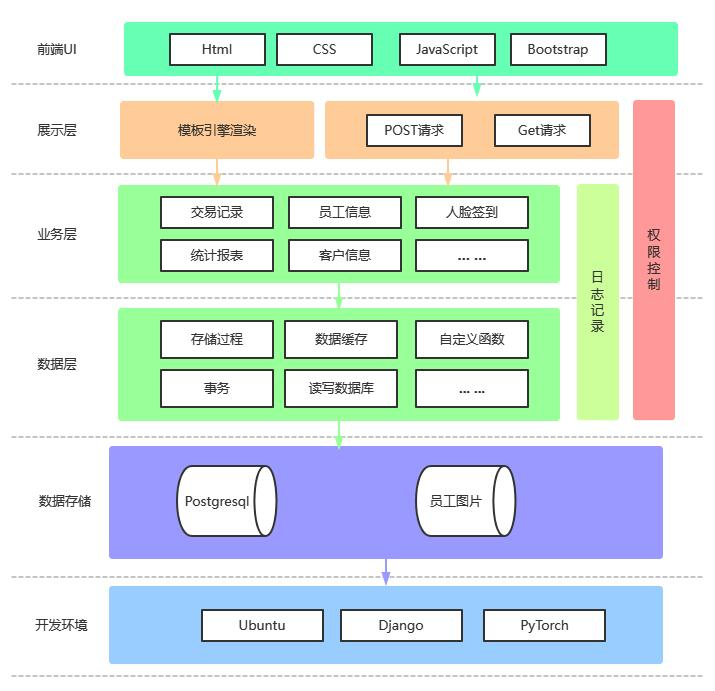
\includegraphics[width=.65\textwidth]{figures/4total.jpg}
%     \caption{系统架构图}
%     \label{fig:sysarc}
% \end{figure}

\begin{figure}[H]
    \centering
    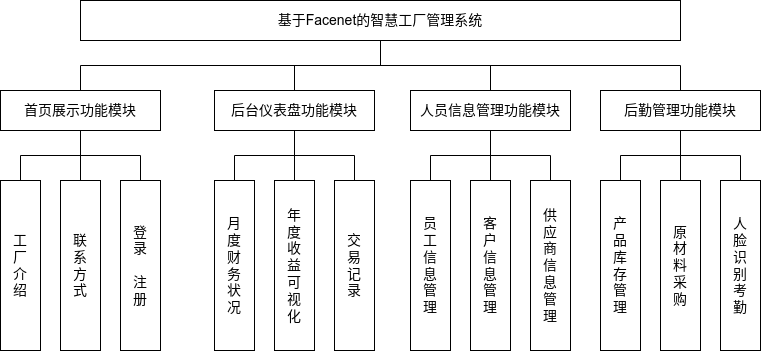
\includegraphics[width=\textwidth]{figures/4funmod.png}
    \caption{总体功能模块图}
    \label{fig:funmod}
\end{figure}

\subsubsection{首页展示功能模块设计}

当客户浏览当前工厂首页页面时,首页页面负责向客户提供工厂介绍功能,其中包括工厂的标语口号、工厂特点介绍、工厂提供服务详情以及联系方式等。在顶部导航栏为人员提供注册登录信息。在注册页面,注册人员需要根据页面提示输出一些必需的个人信息,例如组织名称、电子邮件、电话号码、用户名和密码等。在登录页面,输入管理员用户名以及密码即可进入后台管理页面。

\subsubsection{后台仪表盘功能模块设计}

工厂管理员通过管理账号登录,进入到后台管理页面,根据当前登录用户名,显示一条欢迎信息。在后台管理页面的首页,向管理决策人员展示当前工厂的财务状况,其中包括月度收入、支出和利润,年度收益概况折线图,月度收入概况饼图;在财务状况下方,向管理人员展示最近的入账交易记录以及出账交易记录。

\subsubsection{人员信息管理功能模块设计}

在后台管理页面中,工厂管理员可对当前组织部门的人员进行管理,其中包括客户信息、员工信息以及供应商信息管理等。客户信息有客户姓名、收货地址、联系方式以及相关联的订单详情,管理人员可指定特定客户对其进行下单操作。员工信息还包括了职位、薪资以及所完成的工作详情,管理人员还可以根据产品以及重量对特定员工下达工作任务。供应商信息有供应商姓名、发货地址以及联系方式等。管理人员可根据工厂部门的运营情况,实时对当前人员信息进行管理。

\subsubsection{后勤管理功能模块设计}

1. 产品库存管理:工厂部门管理人员可在后台管理页面,查看当前工厂部门所生产的产品类型以及数量、原材料类型以及数量。客户下单时对产品数量进行更新,管理人员还可指定员工对特定产品进行生成制造,也对产品以及数量进行更新。

2. 原材料采购:当工厂需要订购原材料,管理人员可在订购原材料页面指定供应商、原材料以及数量等信息,进行原材料购买操作。

3. 人脸识别考勤:工厂部门管理人员除了对工厂信息进行管理之外,还需要对员工的考勤进行记录。在考勤页面中,可通过人脸识别功能模块对当前员工进行身份认证,认证通过后,在后勤签到记录表中插入当前员工的签到记录。

\subsection{人脸识别功能模块设计}

本系统结合深度学习人脸识别技术,使用Facenet网络模型进行训练,来实现对员工考勤签到功能。进入到员工考勤页面,首先向管理员展示最近的员工签到表,包含员工姓名以及签到时间。进行人脸签到时,计算人脸图像的embedding编码,与本地员工人脸图像数据库进行比对,得到两者最小距离的员工,并且检查是否小于阈值,通过后便向签到表添加记录。

\subsubsection{构造数据集}

由于新冠疫情的影响,人们在日常出行的时候佩戴口罩是必不可少的。由于佩戴口罩对人脸进行了遮挡,所以在一些基于人脸识别的传统系统受到了很多挑战。所以本系统选择基于用于训练人脸识别的CASIA-Webface的人脸数据集基础之上,使用MaskTheFace工具对数据集进行构造,构造一个模拟佩戴口罩人脸数据集用于训练。CASIA-Webface由10,575位人物共494,414张人脸图像构成,部分人脸图像如图\ref{fig:webface}所示。

\begin{figure}[H]
    \centering
    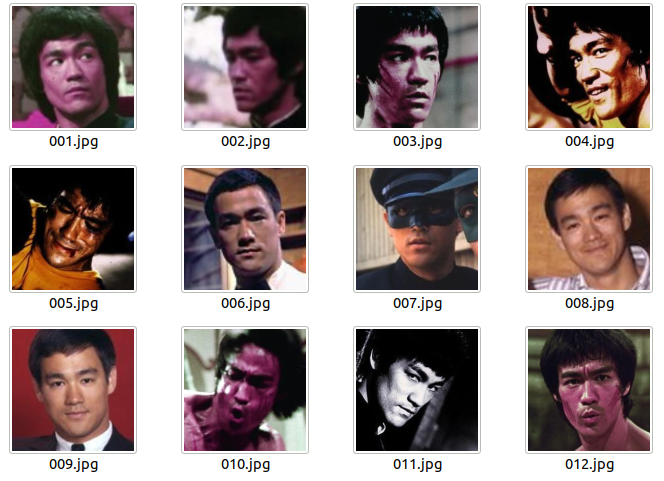
\includegraphics[width=.4\textwidth]{figures/4webface.png}
    \caption{CASIA-Webface人脸数据集部分图像}
    \label{fig:webface}
\end{figure}

训练完神经网络模型之后,使用LFW数据集和MFR2数据集进行测试评估模型的性能,参考模型对人脸识别的准确率。其中LFW是现实世界的涵盖各种自然可变因素的人脸数据集,由5,749位人物共13,233张人脸图像,其中1,680位人物有2张以上的人脸图像,部分人脸图像如图\ref{fig:lfw}所示。MFR2是现实世界的佩戴口罩的人脸数据集,由53位名人和政治家共269张佩戴口罩的人脸图像构成,部分人脸图像如图\ref{fig:mfr2}所示。

\begin{figure}[H]
    \centering
    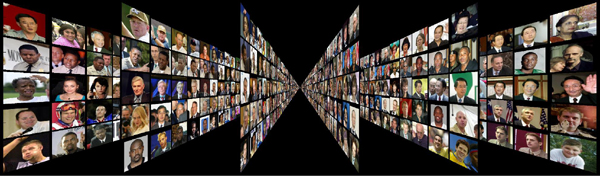
\includegraphics[width=.75\textwidth]{figures/4lfw.jpg}
    \caption{LFW人脸数据集部分图像}
    \label{fig:lfw}
\end{figure}

\begin{figure}[H]
    \centering
    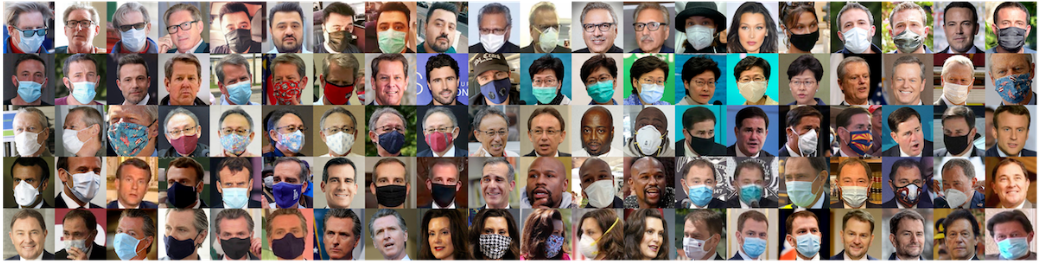
\includegraphics[width=.75\textwidth]{figures/4mfr2.png}
    \caption{MFR2人脸数据集部分图像}
    \label{fig:mfr2}
\end{figure}

\subsubsection{模型设计}

本系统选用Facenet网络模型用于人脸识别,模型整体结构如图\ref{fig:modelarc}所示,其中最左边表示一个批量的图像输入到深度卷积神经网络中,对卷积神经网络的输出进行$L_{2}$ normalization得到人脸图像的embedding编码,之后使用TripletLoss为损失函数进行训练。

\begin{figure}[H]
    \centering
    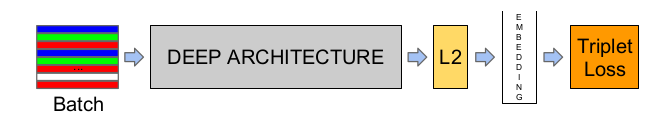
\includegraphics[width=.75\textwidth]{figures/4modelarc.png}
    \caption{模型整体架构图}
    \label{fig:modelarc}
\end{figure}

TripletLoss可以直接反映出人脸验证、识别和聚类所能达到的效果。换句话说,对于一张输入人脸图像$x$映射到特征空间$\mathbb{R}^d$中,通过$f(x)$得到embedding,来使得相同人物的人脸图像之间的平方距离更小(与成像条件相独立),而对于来自于不同人物的图像对之间的平方距离尽可能地大。

\subsubsection{TripletLoss损失函数}

人脸图像的embedding编码由$f(x)\in\mathbb{R}^d$表示,它将一张图像$x$嵌入到一个d维的欧式空间。并且将embedding编码限制到一个d维的超球面,也就是使得$\left \| f(x) \right \| _2=1$。在本模型中,要确保一个特定人物的图像$x_i^a$(anchor)尽可能接近与其相同人物的其它图像$x_i^p$(positive),而与剩余任何一个其他人物的图像$x_i^n$(negative)尽可能远,以上过程如图\ref{fig:tpltll}所示。

\begin{figure}[H]
    \centering
    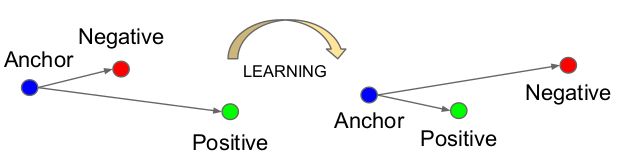
\includegraphics[width=.75\textwidth]{figures/4tpltll.png}
    \caption{TripletLoss训练图}
    \label{fig:tpltll}
\end{figure}

以上过程可以由公式\ref{eq:tpltll}表示,其中,$\alpha$表示正类图像对与负类图像对之间的边距,$\mathcal{T}$表示在训练集中所有可能的三元组集合。

\begin{equation}
    \left\|x_{i}^{a}-x_{i}^{p}\right\|_{2}^{2}+\alpha<\left\|x_{i}^{a}-x_{i}^{n}\right\|_{2}^{2}, \forall\left(x_{i}^{a}, x_{i}^{p}, x_{i}^{n}\right) \in \mathcal{T}
    \label{eq:tpltll}
\end{equation}

由此便可得到要被最小化的损失函数$L$,由公式\ref{eq:loss}表示。

\begin{equation}
    L=\sum_{i}^{N}\left[\left\|f\left(x_{i}^{a}\right)-f\left(x_{i}^{p}\right)\right\|_{2}^{2}-\left\|f\left(x_{i}^{a}\right)-f\left(x_{i}^{n}\right)\right\|_{2}^{2}+\alpha\right]_{+}
    \label{eq:loss}
\end{equation}

\subsubsection{模型评估性能指标}

所有的相同人物的人脸图像对$(i,j)$被表示为$\mathcal{P}_{\text {same}}$,不同人物的人脸图像对表示为$\mathcal{P}_{\text {diff}}$。之后,定义所有true accept的集合,由公式\ref{eq:ta}表示有人脸对$(i,j)$被正确地分为同一位人物,其中$D\left(x_{i}, x_{j}\right)$表示为一对图像之间的距离,$d$表示为距离阈值。

\begin{equation}
    \mathrm{TA}(d)=\left\{(i, j) \in \mathcal{P}_{\text {same }}, \text { with } D\left(x_{i}, x_{j}\right) \leq d\right\}
    \label{eq:ta}
\end{equation}

相似地,可以定义false accept,公式为\ref{eq:fa}。

\begin{equation}
    \mathrm{FA}(d)=\left\{(i, j) \in \mathcal{P}_{\text {diff }}, \text { with } D\left(x_{i}, x_{j}\right) \leq d\right\}
    \label{eq:fa}
\end{equation}

对于一个给定的人脸距离阈值$d$,验证率(validation rate)$VAL(d)$和错误接受率(false accept rate)$FAR(d)$被定义为公式\ref{eq:valfar}所示。

\begin{equation}
    \operatorname{VAL}(d)=\frac{|\mathrm{TA}(d)|}{\left|\mathcal{P}_{\text {same }}\right|}, \quad \operatorname{FAR}(d)=\frac{|\mathrm{FA}(d)|}{\left|\mathcal{P}_{\text {diff }}\right|}
    \label{eq:valfar}
\end{equation}

\subsection{数据库设计}

\subsubsection{逻辑设计}

从工厂信息管理着手,该系统所涉及到的实体有账户实体、员工实体、工作任务实体、薪资实体、客户实体、产品订单实体、供应商实体、产品实体、原材料订单实体、交易记录实体以及签到记录实体等。以下为该系统关键实体描述。

1. 员工实体:员工实体所包含的属性有员工姓名、基本工资、奖金、薪资共计、本月是否已支付薪资、最后一次更新薪资日期、职称、地址、电话号码、出生日期、入职日期以及性别。如图\ref{fig:4emplyerf}所示为员工的实体属性图。

\begin{figure}[H]
    \centering
    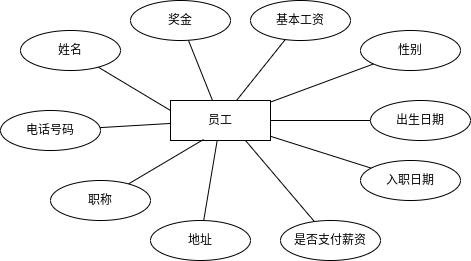
\includegraphics[width=.65\textwidth]{figures/4emplyerf.png}
    \caption{员工实体属性图}
    \label{fig:4emplyerf}
\end{figure}

2. 账号实体:账号实体也可看作为管理员实体,其中所涉及到的属性有组织名称、电话号码、电子邮件、用户名以及密码。如图\ref{fig:4acterf}所示为管理员的实体属性图。

\begin{figure}[H]
    \centering
    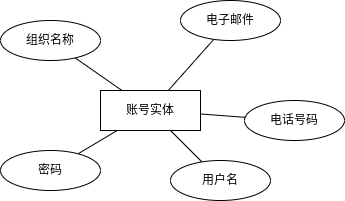
\includegraphics[width=.45\textwidth]{figures/4acterf.png}
    \caption{账号实体属性图}
    \label{fig:4acterf}
\end{figure}

3. 产品实体:产品实体所包含的属性有名称、成本、报酬和重量等。如图\ref{fig:4prdcterf}所示为产品的实体属性图。

\begin{figure}[H]
    \centering
    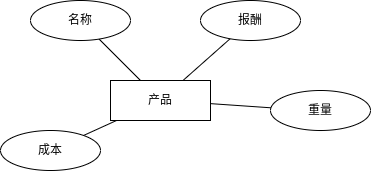
\includegraphics[width=.45\textwidth]{figures/4prdcterf.png}
    \caption{产品实体属性图}
    \label{fig:4prdcterf}
\end{figure}

4. 交易记录实体:交易记录所包含的属性有交易金额、交易描述、类型和交易日期,其中类型包括入账和出账。如图\ref{fig:4tscterf}所示为交易记录的实体属性图。

\begin{figure}[H]
    \centering
    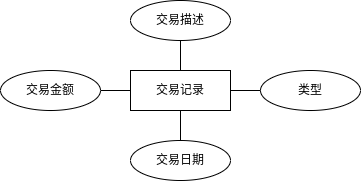
\includegraphics[width=.45\textwidth]{figures/4tscterf.png}
    \caption{交易记录实体属性图}
    \label{fig:4tscterf}
\end{figure}

5. 原材料实体:原材料所涉及到的属性有原材料名称、目前可用重量、材料成本和制造产品百分比。如图\ref{fig:4rmtraerf}所示为原材料的实体属性图。

\begin{figure}[H]
    \centering
    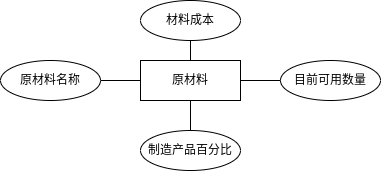
\includegraphics[width=.45\textwidth]{figures/4rmtraerf.png}
    \caption{原材料实体属性图}
    \label{fig:4rmtraerf}
\end{figure}

6. 薪资实体:薪资所包含的属性有员工、基本工资、奖金、共计和支付日期等。如图\ref{fig:4slrerf}所示为薪资的实体属性图。

\begin{figure}[H]
    \centering
    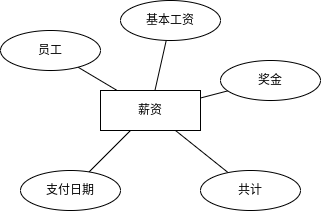
\includegraphics[width=.45\textwidth]{figures/4slrerf.png}
    \caption{薪资实体属性图}
    \label{fig:4slrerf}
\end{figure}

7. 客户:客户所涉及到信息只需客户姓名、手机号码和收货地址。如图\ref{fig:4cstmerf}所示为客户的实体属性图。

\begin{figure}[H]
    \centering
    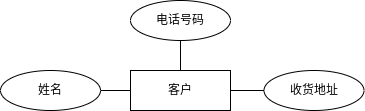
\includegraphics[width=.45\textwidth]{figures/4cstmerf.png}
    \caption{客户实体属性图}
    \label{fig:4cstmerf}
\end{figure}

8. 订单:订单所包含的属性有客户、下单日期、送达日期、是否送达以及总共数量。如图\ref{fig:4oderf}所示为客户的实体属性图。

\begin{figure}[H]
    \centering
    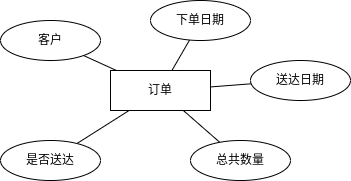
\includegraphics[width=.45\textwidth]{figures/4oderf.png}
    \caption{订单实体属性图}
    \label{fig:4oderf}
\end{figure}

之后将所有独立的实体属性图进行基数定义关系,其中包含在客户对某个产品进行下单时,定义客户与产品之间的多对多关系的订单表;在员工生产某一个产品时产出的多对多关系的工作表;工厂管理账户实体对员工和客户等信息进行管理产生的一对多关系。综上,系统的整体E--R图如图\ref{fig:4totalerf}所示。

\begin{figure}[H]
    \centering
    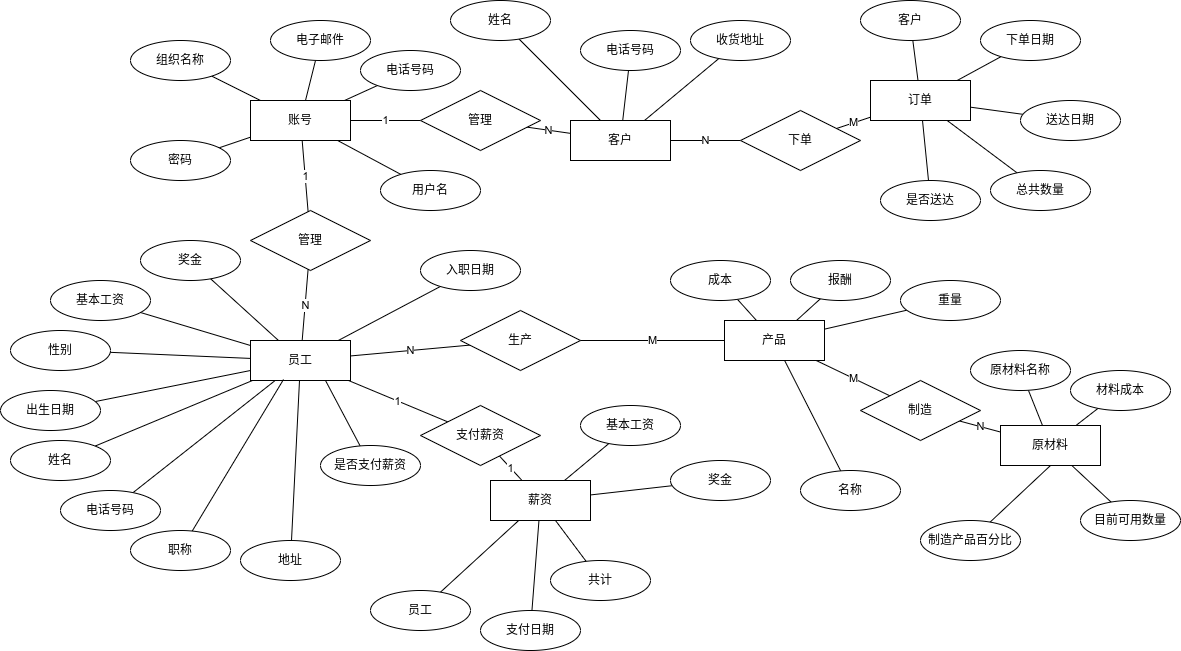
\includegraphics[width=\textwidth]{figures/4totalerf.png}
    \caption{系统E--R图}
    \label{fig:4totalerf}
\end{figure}

\subsubsection{物理设计}

在工厂管理中,首先要对三种不同的实体人物进行抽象,有员工信息、客户信息以及供应商信息。分别对三种实体信息进行抽象抽取,设计数据库关系,如表\ref{tab:emp}所示,给出了员工信息的关系表。

\begin{table}[H]
    \centering
    \zihao{5}
    \caption{员工信息设计表}
    \label{tab:emp}
    \begin{tabularx}{.85\textwidth}{X<{\centering}X<{\centering}X<{\centering}X<{\centering}}
        \toprule
        字段名 & 数据类型 & 默认值 & 描述信息 \\
        \midrule
        name & CharField & NULL & 员工姓名 \\
        basicSalary & DecimalField & 0 & 基本工资 \\
        bonus & DecimalField & 0 & 奖金 \\
        total & DecimalField & 0 & 工资共计 \\
        isPaid & BooleanField & False & 是否支付薪资 \\
        lastSalary & DateField & NULL & 薪资更新日期 \\
        designation & CharField & 其他 & 职称 \\
        address & CharField & NULL & 员工地址 \\
        phone & CharField & NULL & 电话号码 \\
        dob & DateField & NULL & 出生日期 \\
        doj & DateField & NULL & 入职日期 \\
        gender & IntegerField & 2 & 性别 \\
        \bottomrule
    \end{tabularx}
\end{table}

对后勤信息管理部分进行抽象设计,有产品信息、原材料信息以及员工考勤的签到表。分别对产品和原材料的实体信息进行抽象并设计数据库关系表,如表\ref{tab:product}所示,给出了产品信息的关系表。

\begin{table}[H]
    \centering
    \zihao{5}
    \caption{产品信息设计表}
    \label{tab:product}
    \begin{tabularx}{.85\textwidth}{X<{\centering}X<{\centering}X<{\centering}X<{\centering}}
        \toprule
        字段名 & 数据类型 & 默认值 & 描述信息 \\
        \midrule
        name & CharField & NULL & 产品名称 \\
        cost & DecimalField & NULL & 产品成本 \\
        wages & DecimalField & NULL & 产品利润 \\
        weight & DecimalField & NULL& 产品重量 \\
        \bottomrule
    \end{tabularx}
\end{table}

之后将所有独立的实体表进行定义基数关系,其中包含在客户对某个产品进行下单时,定义客户表和产品表之间的多对多关系的订单表;在员工生产某一个产品时就会有多对多关系的工作表;供应商对某一种原材料进行供应时的多对多的供应表等,如图\ref{fig:er}所示,展示本系统关键实体的的E-R关系图。

\begin{figure}[H]
    \centering
    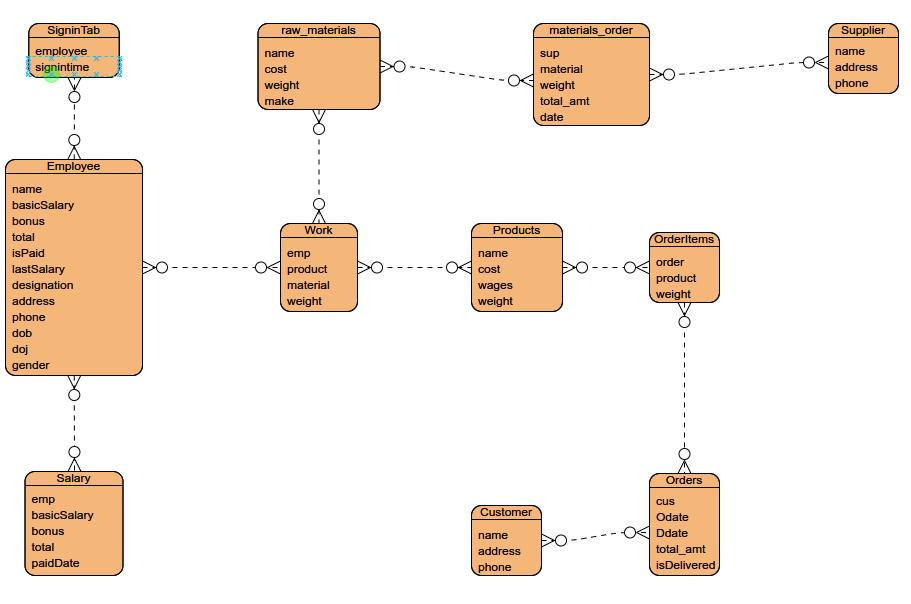
\includegraphics[width=.75\textwidth]{figures/4er.jpg}
    \caption{系统关键实体E-R图}
    \label{fig:er}
\end{figure}
